\newpage
\section {Výsledky}
\label{results}
V nasledujúcej kapitole sú rozobraté dosiahnuté výsledky. Na tie je nutné pozrieť sa z dvoch strán, najprv z pohľadu neurónovej siete a toho, ako dobre sa neurónová sieť dokázala naučiť predikovať na predložených dátach. Potom z pohľadu kvality predikcií a ich porovnania s inými riešeniami použitím metrík na evaluáciu modelov vizuálnej pozornosti. 

\subsection{Evaluácia modelu neurónovej siete}
\label{evaluation}
Na evaluáciu toho, ako dobre bola sieť schopná naučiť sa predikovať sme použili jednoduchý priemer chýb predikcií v jednotlivých bodoch heatmapy.
Ten potom podľa očakávania klesal počas tréningu aj validácie štandardne, ako bolo ukázané na grafoch v časti \ref{model_graph}. Jeho hodnota bola pri testovaní na testovacom datasete 0.2066. Vzhľadom na to, že pri trénovaní na 3/4 datasetu bola chyba 0.2511, predpokladáme, že ďalšie zlepšenie predikcií a zníženie chyby by bolo možné dosiahnuť väčším množstvom dát.

\subsection{Metriky používané na ohodnotenie modelov vizuálnej pozornosti}
\label{metric}
Tradične sa tieto modely evaluujú vzhľadom na pohyb očí, resp. samotné fixácie. K tomu slúži značný počet rôzne fungujúcich metrík\cite{metriky}, najpoužívanejšie sú:

\begin{itemize}

	\item NSS - Normalizovaná cesta pútavosti (z angl. Normalized Scanpath Saliency). Využíva priemer hodnôt pútavosti na \textit{n} fixácií v normalizovanej mape podľa nasledovného vzorca: 
	
	\begin{equation}
	\frac{1}{n} \sum_{i=1}^{n} \frac{s(x_{h}^{i}, y_{h}^{i}) - \mu_{s}}{\sigma _{s}}
	\end{equation}
	
	\item AUC - Oblasť pod ROC krivkou (z angl. Area Under the ROC Curve).
	Ľudské fixácie sú považované za pozitívnu sadu a niektoré body na obrázku sú vybrané ako negatívna sada. K mape pútavosti je potom pristupované ako k binárnemu klasifikátoru na separáciu pozitívnych vzorkov od negatívnych. Presnosť podľa tejto metriky je daná nasledovne: 
	
	\begin{itemize}
		
		\item 0.90 - 1 = výborná
		\item 0.80 - 0.90 = dobrá
		\item 0.70 - 0.80 = priemerná
		\item 0.60 - 0.70 = slabá
		\item 0.50 - 0.60 = veľmi slabá
		
	\end{itemize}
	
	\item sAUC - Zamiešaná oblasť pod ROC krivkou (z angl. shuffled Area Under the ROC Curve) je mierna modifikácia vyššie uvedenej metriky, kedy ako negatívna sada nie sú vybrané len niektoré body, ale všetky body, ktoré nie sú ľudskými fixáciami, sú považované za negatívne. Určenie presnosti na základe hodnôt je rovnaké ako pri AUC. 
	
	\item CC - Korelačný koeficient, určuje prakticky podobnosť v tomto prípade dvoch máp výraznosti, kde jedna je výsledok modelu vizuálnej pozornosti a druhá je reálna mapa vypočítaná z fixácií. 
	
	\begin{equation}
	CC (s, h) = \frac{cov(s, h)}{\sigma_{s} \sigma _{h}}
	\end{equation}
\end{itemize}

Z vyššie popísaných metrík sme k finálnej evaluácii a porovnaniu s inými riešeniami použili tri, a to CC, sAUC a NSS.
  
\subsection{Porovnanie s inými riešeniami}
\label{comparison}
Výsledné predikcie nášho riešenia sme porovnali s Itti-ho modelom vizuálnej pozornosti (popísaný v \ref{itti}) pomocou vyššie uvedených metrík. Metriky boli počítané na nových testovacích dátach, ktoré naša neurónová sieť doteraz nevidela. Je však nutné spomenúť, že Itti-ho model nie je primárne zameraný na určovanie vizuálne pútavých častí grafických rozhraní web stránok, jedná sa skôr o všeobecný model vizuálnej pozornosti. Porovnanie a hodnoty metrík je možné násť v tabuľke \ref{itti_vs_my}.

\begin{table}[H]
	%\begin{minipage}{\textwidth}
		\centering
		\caption[Porovnanie s Itti-ho modelom vizuálnej pozornosti]{Porovnanie hodnôt metrík pre Itti-ho a náš model}
		\label{itti_vs_my}
		\begin{tabular}{{ | p{2cm} |  p{3cm} |  p{3cm} |  p{3cm} |  }}
			\hline
			& \textbf{Itti-ho model} &  \textbf{Náš model} \\ \hline
			CC & 0.4535 & 0.6620  \\ \hline
			sAUC & 0.5785 & 0.7163 \\ \hline
			NSS & 0.3309 & 0.6998  \\ \hline
		\end{tabular}
		
	%\end{minipage}
\end{table}

Z tabuľky je vidieť, že náš model bol podľa metrík schopný predikovať o niečo presnejšie mapy výraznosti ako Itti-ho model. Na obrázku \ref{fig:itti_vs_my} je zobrazené porovnanie predikcií formou vizualizácie. 

	\begin{figure}[H]
		\begin{center}
			
\includegraphics[scale=1, width = 4cm, height = 2.5cm]{original_2.png}
			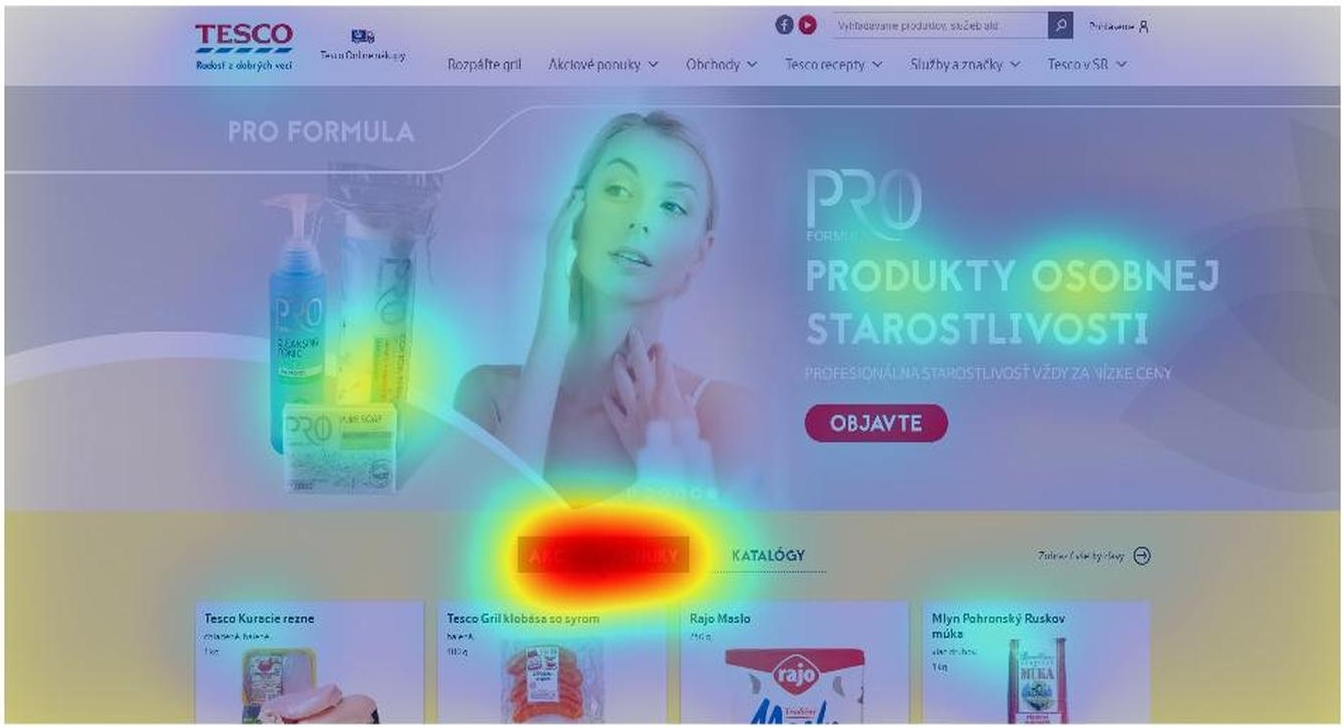
\includegraphics[scale=1, width = 4cm, height = 2.5cm]{itti_2.jpg}
			
\includegraphics[scale=1, width = 4cm, height = 2.5cm]{prediction_for_tesco.jpg}			
		\end{center}
		\begin{center}
			
\includegraphics[scale=1, width = 4cm, height = 2.5cm]{final_test_3.png}
			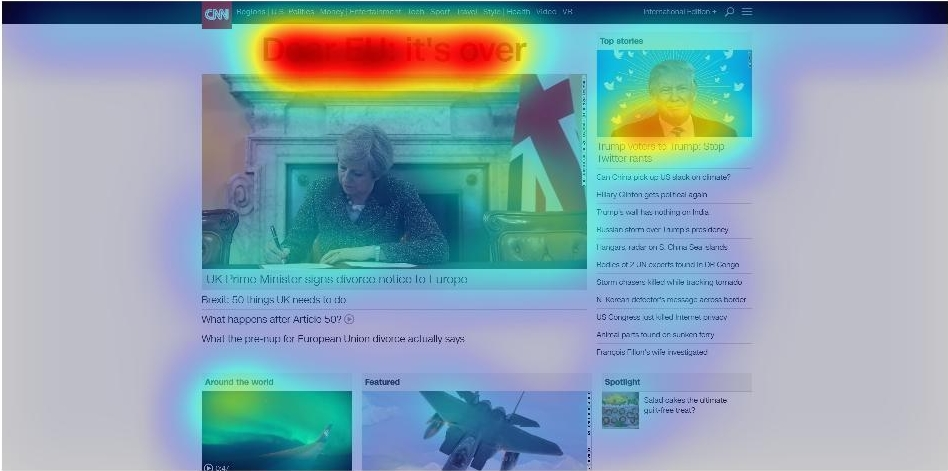
\includegraphics[scale=1, width = 4cm, height = 2.5cm]{itti_cnn.jpg}
			
\includegraphics[scale=1, width = 4cm, height = 2.5cm]{prediction_for_cnn.jpg}			
		\end{center}
		\begin{center}
			
\includegraphics[scale=1, width = 4cm, height = 2.5cm]{hm_31.png}
			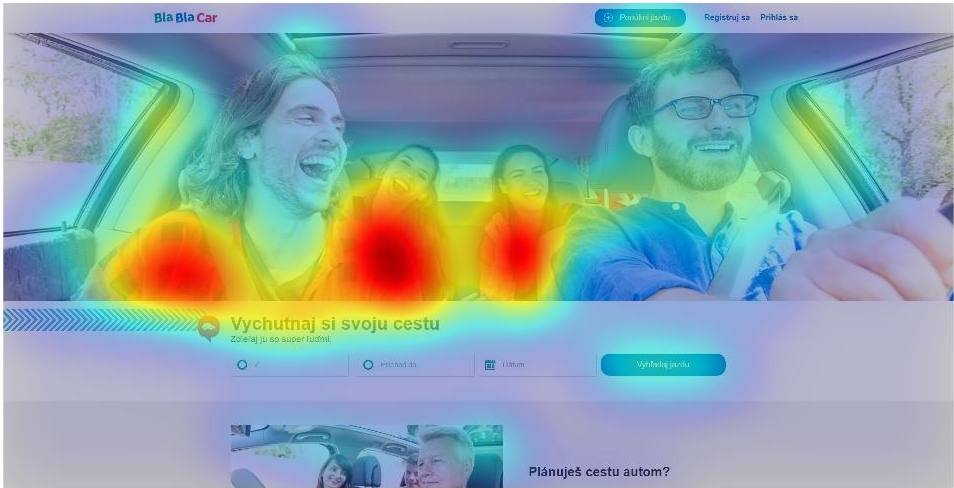
\includegraphics[scale=1, width = 4cm, height = 2.5cm]{itti_blablacar.jpg}
			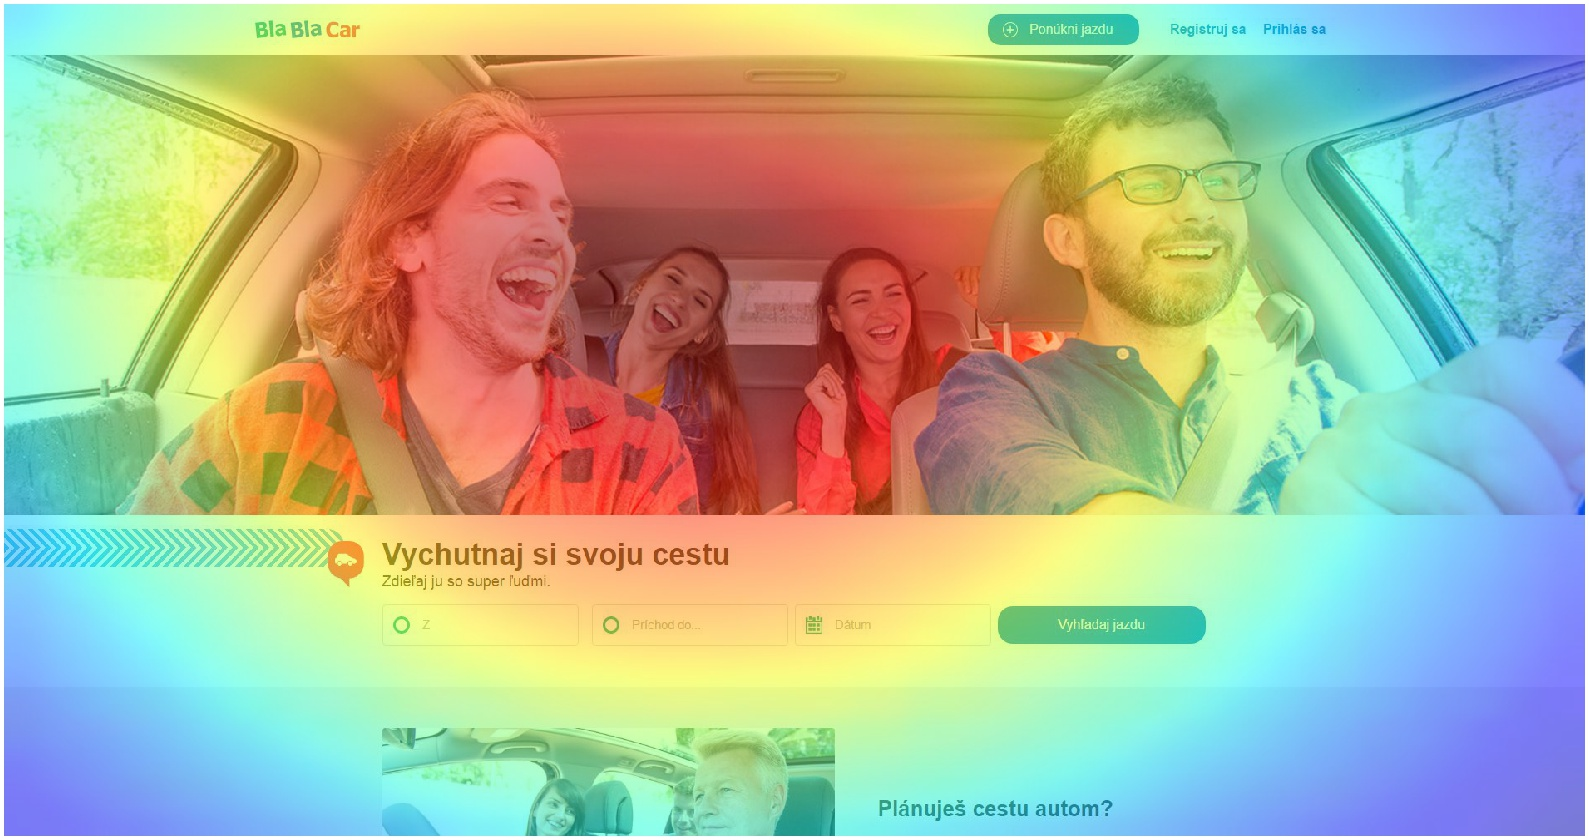
\includegraphics[scale=1, width = 4cm, height = 2.5cm]{prediction_for_blablacar.JPG}			
		\end{center}
		\begin{center}
			
\includegraphics[scale=1, width = 4cm, height = 2.5cm]{original_5.png}
			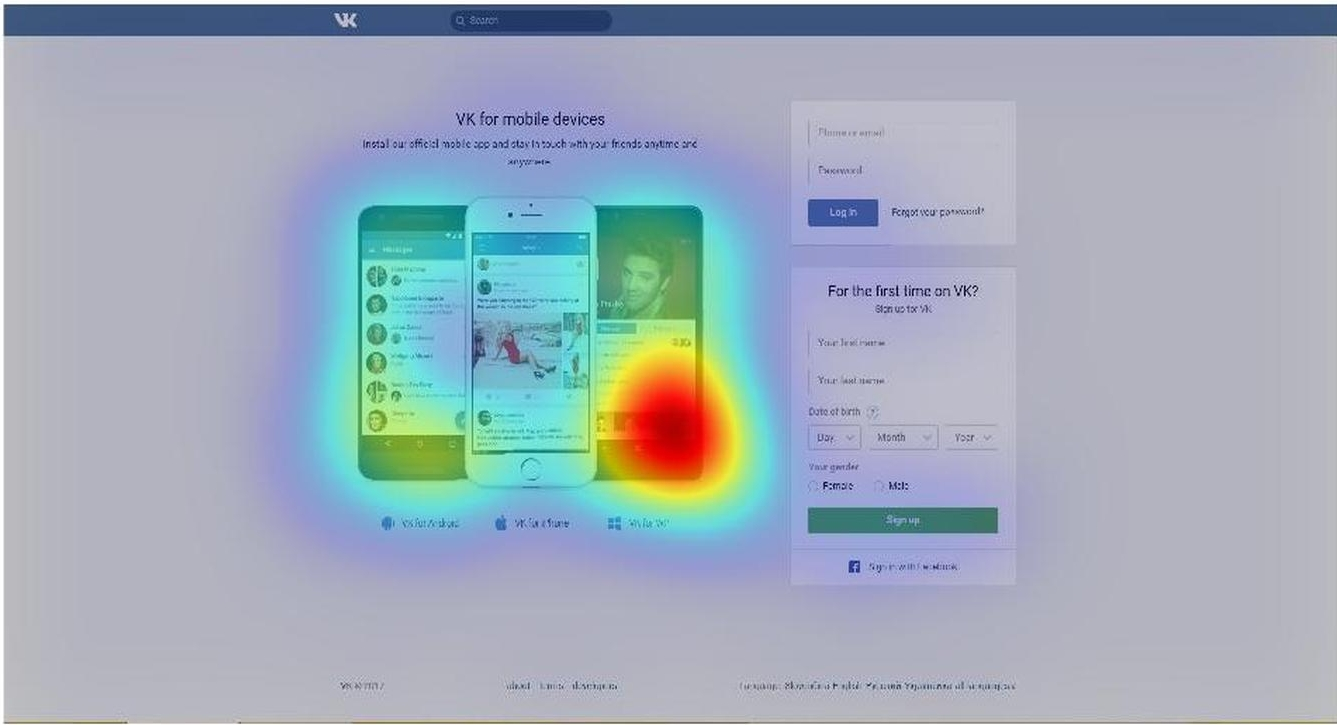
\includegraphics[scale=1, width = 4cm, height = 2.5cm]{itti_5.jpg}
			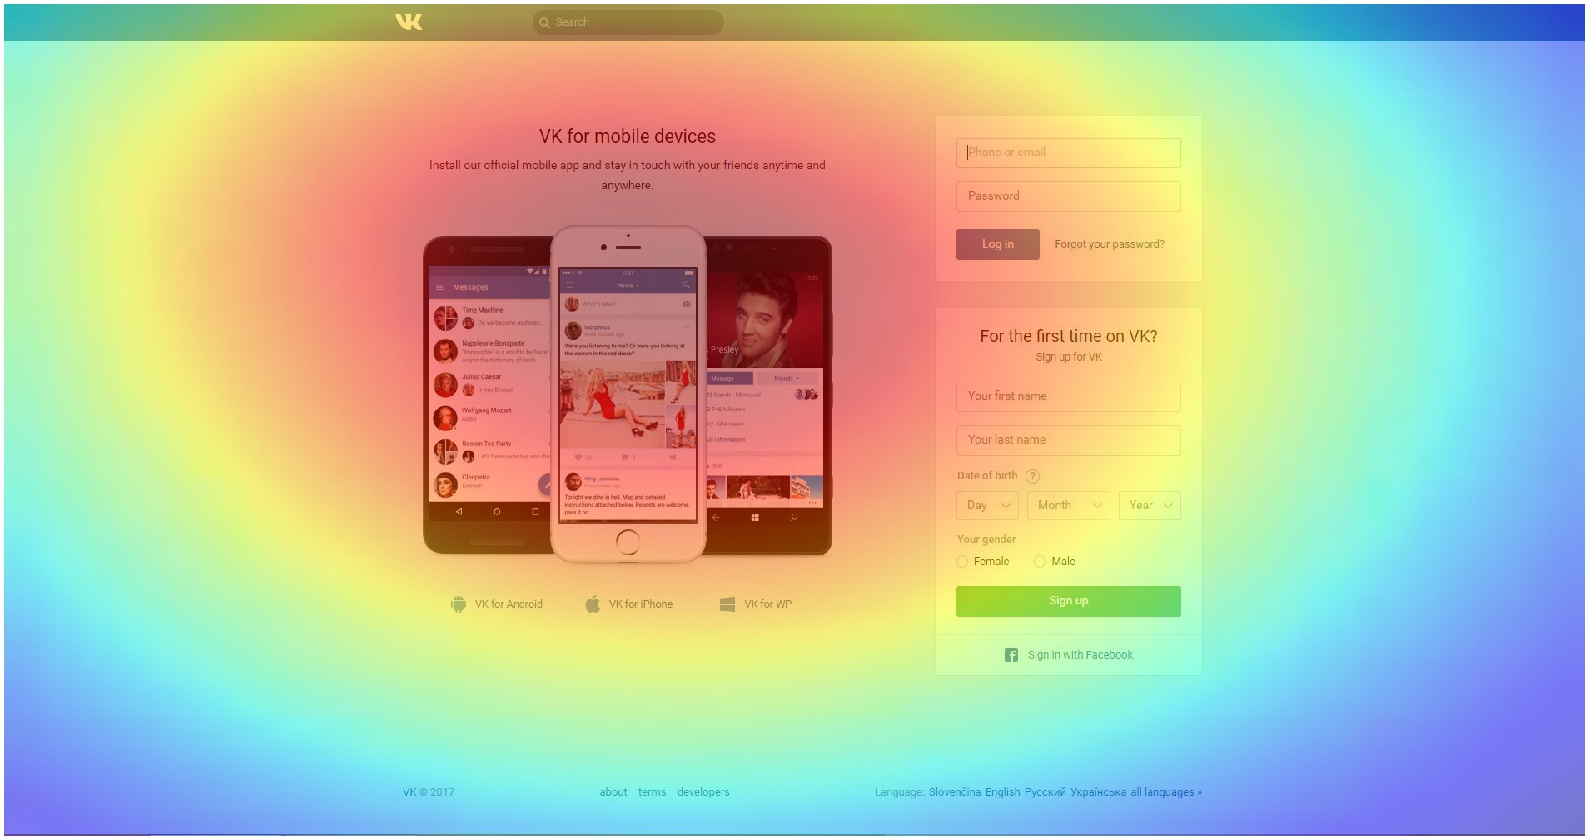
\includegraphics[scale=1, width = 4cm, height = 2.5cm]{prediction_for_vk.jpg}			
		\end{center}
		\caption[Náš model vs. Itti-ho model]{
			Grafická vizualizácia porovnania predikciíí Itt-ho modelu s naším. Vľavo mapy výraznosti vypočítané z reálnych fixácií ľudí, v strede predikcia pomocou Itti-ho modelu, vpravo predikcia nášho modelu.
		}\label{fig:itti_vs_my}
	\end{figure}

Na obrázku je možné pozorovať, že v niektorých situáciách je náš model presnejší, v iných nie. Naša neurónová sieť sa naučila predikovať primárne do strednej hornej oblasti, čo však na väčšine typov stránok je aj reálne prvá oblasť, ktorú vnímame. 

Najideálnejšie by bolo náš model porovnať s modelom od Chengyao Shen a Qi Zhao\cite{singapur_model}, popísaným v časti \ref{singapur}, ale ich dataset ani riešenie nie sú verejne dostupné. Hodnoty metrík preto nie sú vypočítané na tých istých dátach a porovnanie môže byť trochu zavádzajúce, prakticky ale náš model dosiahol hodnoty CC zhruba o 0.06 vyššie, sAUC je na tej istej úrovni a NSS má náš model o polovicu nižší, je to jediná metrika kde sme výrazne horší ako ich model. 